%% Template for the submission to:
%%   The Annals of Applied Statistics [AOAS]
%%
%%%%%%%%%%%%%%%%%%%%%%%%%%%%%%%%%%%%%%%%%%%%%%
%% In this template, the places where you   %%
%% need to fill in your information are     %%
%% indicated by '???'.                      %%
%%                                          %%
%% Please do not use \input{...} to include %%
%% other tex files. Submit your LaTeX       %%
%% manuscript as one .tex document.         %%
%%%%%%%%%%%%%%%%%%%%%%%%%%%%%%%%%%%%%%%%%%%%%%

\documentclass[aoas]{imsart}\usepackage[]{graphicx}\usepackage[]{xcolor}
% maxwidth is the original width if it is less than linewidth
% otherwise use linewidth (to make sure the graphics do not exceed the margin)
\makeatletter
\def\maxwidth{ %
  \ifdim\Gin@nat@width>\linewidth
    \linewidth
  \else
    \Gin@nat@width
  \fi
}
\makeatother

\definecolor{fgcolor}{rgb}{0.345, 0.345, 0.345}
\newcommand{\hlnum}[1]{\textcolor[rgb]{0.686,0.059,0.569}{#1}}%
\newcommand{\hlstr}[1]{\textcolor[rgb]{0.192,0.494,0.8}{#1}}%
\newcommand{\hlcom}[1]{\textcolor[rgb]{0.678,0.584,0.686}{\textit{#1}}}%
\newcommand{\hlopt}[1]{\textcolor[rgb]{0,0,0}{#1}}%
\newcommand{\hlstd}[1]{\textcolor[rgb]{0.345,0.345,0.345}{#1}}%
\newcommand{\hlkwa}[1]{\textcolor[rgb]{0.161,0.373,0.58}{\textbf{#1}}}%
\newcommand{\hlkwb}[1]{\textcolor[rgb]{0.69,0.353,0.396}{#1}}%
\newcommand{\hlkwc}[1]{\textcolor[rgb]{0.333,0.667,0.333}{#1}}%
\newcommand{\hlkwd}[1]{\textcolor[rgb]{0.737,0.353,0.396}{\textbf{#1}}}%
\let\hlipl\hlkwb

\usepackage{framed}
\makeatletter
\newenvironment{kframe}{%
 \def\at@end@of@kframe{}%
 \ifinner\ifhmode%
  \def\at@end@of@kframe{\end{minipage}}%
  \begin{minipage}{\columnwidth}%
 \fi\fi%
 \def\FrameCommand##1{\hskip\@totalleftmargin \hskip-\fboxsep
 \colorbox{shadecolor}{##1}\hskip-\fboxsep
     % There is no \\@totalrightmargin, so:
     \hskip-\linewidth \hskip-\@totalleftmargin \hskip\columnwidth}%
 \MakeFramed {\advance\hsize-\width
   \@totalleftmargin\z@ \linewidth\hsize
   \@setminipage}}%
 {\par\unskip\endMakeFramed%
 \at@end@of@kframe}
\makeatother

\definecolor{shadecolor}{rgb}{.97, .97, .97}
\definecolor{messagecolor}{rgb}{0, 0, 0}
\definecolor{warningcolor}{rgb}{1, 0, 1}
\definecolor{errorcolor}{rgb}{1, 0, 0}
\newenvironment{knitrout}{}{} % an empty environment to be redefined in TeX

\usepackage{alltt}

%% Packages
\RequirePackage{amsthm,amsmath,amsfonts,amssymb}
\RequirePackage[authoryear]{natbib}
\RequirePackage[colorlinks,citecolor=blue,urlcolor=blue]{hyperref}
\RequirePackage{graphicx, booktabs, hyperref}

%\RequirePackage[colorlinks,citecolor=blue,urlcolor=blue]{hyperref}%% uncomment this for coloring bibliography citations and linked URLs

\startlocaldefs
%%%%%%%%%%%%%%%%%%%%%%%%%%%%%%%%%%%%%%%%%%%%%%
%%                                          %%
%% Uncomment next line to change            %%
%% the type of equation numbering           %%
%%                                          %%
%%%%%%%%%%%%%%%%%%%%%%%%%%%%%%%%%%%%%%%%%%%%%%
%\numberwithin{equation}{section}
%%%%%%%%%%%%%%%%%%%%%%%%%%%%%%%%%%%%%%%%%%%%%%
%%                                          %%
%% For Axiom, Claim, Corollary, Hypothesis, %%
%% Lemma, Theorem, Proposition              %%
%% use \theoremstyle{plain}                 %%
%%                                          %%
%%%%%%%%%%%%%%%%%%%%%%%%%%%%%%%%%%%%%%%%%%%%%%
%\theoremstyle{plain}
%\newtheorem{???}{???}
%\newtheorem*{???}{???}
%\newtheorem{???}{???}[???]
%\newtheorem{???}[???]{???}
%%%%%%%%%%%%%%%%%%%%%%%%%%%%%%%%%%%%%%%%%%%%%%
%%                                          %%
%% For Assumption, Definition, Example,     %%
%% Notation, Property, Remark, Fact         %%
%% use \theoremstyle{remark}                %%
%%                                          %%
%%%%%%%%%%%%%%%%%%%%%%%%%%%%%%%%%%%%%%%%%%%%%%
%\theoremstyle{remark}
%\newtheorem{???}{???}
%\newtheorem*{???}{???}
%\newtheorem{???}{???}[???]
%\newtheorem{???}[???]{???}
%%%%%%%%%%%%%%%%%%%%%%%%%%%%%%%%%%%%%%%%%%%%%%
%% Please put your definitions here:        %%
%%%%%%%%%%%%%%%%%%%%%%%%%%%%%%%%%%%%%%%%%%%%%%

\endlocaldefs
\IfFileExists{upquote.sty}{\usepackage{upquote}}{}
\begin{document}

%\SweaveOpts{concordance=TRUE}

\begin{frontmatter}
%%%%%%%%%%%%%%%%%%%%%%%%%%%%%%%%%%%%%%%%%%%%%%
%%                                          %%
%% Enter the title of your article here     %%
%%                                          %%
%%%%%%%%%%%%%%%%%%%%%%%%%%%%%%%%%%%%%%%%%%%%%%
\title{Spatial Models for Canadian Temperature Inference}
\runtitle{STAT444: Final Project}

\begin{aug}
%%%%%%%%%%%%%%%%%%%%%%%%%%%%%%%%%%%%%%%%%%%%%%%
%% Only one address is permitted per author. %%
%% Only division, organization and e-mail is %%
%% included in the address.                  %%
%% Additional information can be included in %%
%% the Acknowledgments section if necessary. %%
%% ORCID can be inserted by command:         %%
%% \orcid{0000-0000-0000-0000}               %%
%%%%%%%%%%%%%%%%%%%%%%%%%%%%%%%%%%%%%%%%%%%%%%%

\author[A]{\fnms{Bryan}~\snm{Zang}\ead[label=e1]{bszang@uwaterloo.ca}}

%%%%%%%%%%%%%%%%%%%%%%%%%%%%%%%%%%%%%%%%%%%%%%
%% Addresses                                %%
%%%%%%%%%%%%%%%%%%%%%%%%%%%%%%%%%%%%%%%%%%%%%%
\address[A]{Department of Statistics,
University of Waterloo\printead[presep={,\ }]{e1}}

\end{aug}

\begin{abstract}
Climate change has been a hot topic over the past few decades and remains to be so; an important factor to measure then is temperature. We will show that under some naive assumptions, the global additive model provides the most interpretable results in understanding the spatial variance of Canadian temperature change over some defined regions.
\end{abstract}

\end{frontmatter}
%%%%%%%%%%%%%%%%%%%%%%%%%%%%%%%%%%%%%%%%%%%%%%
%% Please use \tableofcontents for articles %%
%% with 50 pages and more                   %%
%%%%%%%%%%%%%%%%%%%%%%%%%%%%%%%%%%%%%%%%%%%%%%
%\tableofcontents

%%%%%%%%%%%%%%%%%%%%%%%%%%%%%%%%%%%%%%%%%%%%%%
%%%% Main text entry area:
\section{Introduction}\hfill\\

With the progression in science and technology, it has been evident over the past decades that human activity has caused significant amounts of greenhouse gas (GHG) emissions. These GHG emissions trap radiation and heat from the sun, leading to global warming and climate change. To measure the rate and effect of these GHG emissions, we can use temperature as it is a key factor influencing various parts of the regional and global ecosystem \footnote{\cite{b1}}. We wish to model the temperature change in Canada hoping to identify possible variances in the regional data and if so, why? This will be done by fitting a selected model to the regional data and assessing the fit of the model.

\section{Data}\hfill\\

Our data comes from the \texttt{R} package \texttt{gamair} \footnote{\cite{b2}}, it is the \texttt{CanWeather} dataset which is a dataset describing Canadian temperature (averaged over the years 1960-1994) throughout a year at 35 different locations. There is a column of integers denoting the day in the year (1-365), a numerical column for the mean temperature for that day in Celsius, a column of categorical data denoting the general location (Arctic, Atlantic, Continental, or Pacific), a numerical column denoting the location latitude, and another categorical column of location names. We conducted some brief exploratory data analysis to better understand the data and temperature arises as the response variable of interest, and covariates such as time and region appear to be interesting in the sense that we are able to partition data into portions local to some variable (i.e., the temperature change in $x$ days or the overall temperature model in the Atlantic region). Conducting a summary of the data we have the table below
\begin{knitrout}
\definecolor{shadecolor}{rgb}{0.969, 0.969, 0.969}\color{fgcolor}\begin{table}[!h]
\centering\begingroup\fontsize{10}{12}\selectfont

\begin{tabular}[t]{lllll}
\toprule
  &      time &       T &         region &    latitude\\
\midrule
 & Min.   :  1 & Min.   :-34.800 & Arctic     :1095 & Min.   :42.48\\
 & 1st Qu.: 92 & 1st Qu.: -6.700 & Atlantic   :5475 & 1st Qu.:45.58\\
 & Median :183 & Median :  4.100 & Continental:4380 & Median :49.53\\
 & Mean   :183 & Mean   :  1.878 & Pacific    :1825 & Mean   :51.84\\
 & 3rd Qu.:274 & 3rd Qu.: 12.600 & NA & 3rd Qu.:54.47\\
 & Max.   :365 & Max.   : 22.800 & NA & Max.   :74.41\\
\bottomrule
\end{tabular}
\endgroup{}
\end{table}

\end{knitrout}
\newpage

\noindent and the following plots
\begin{knitrout}
\definecolor{shadecolor}{rgb}{0.969, 0.969, 0.969}\color{fgcolor}

{\centering 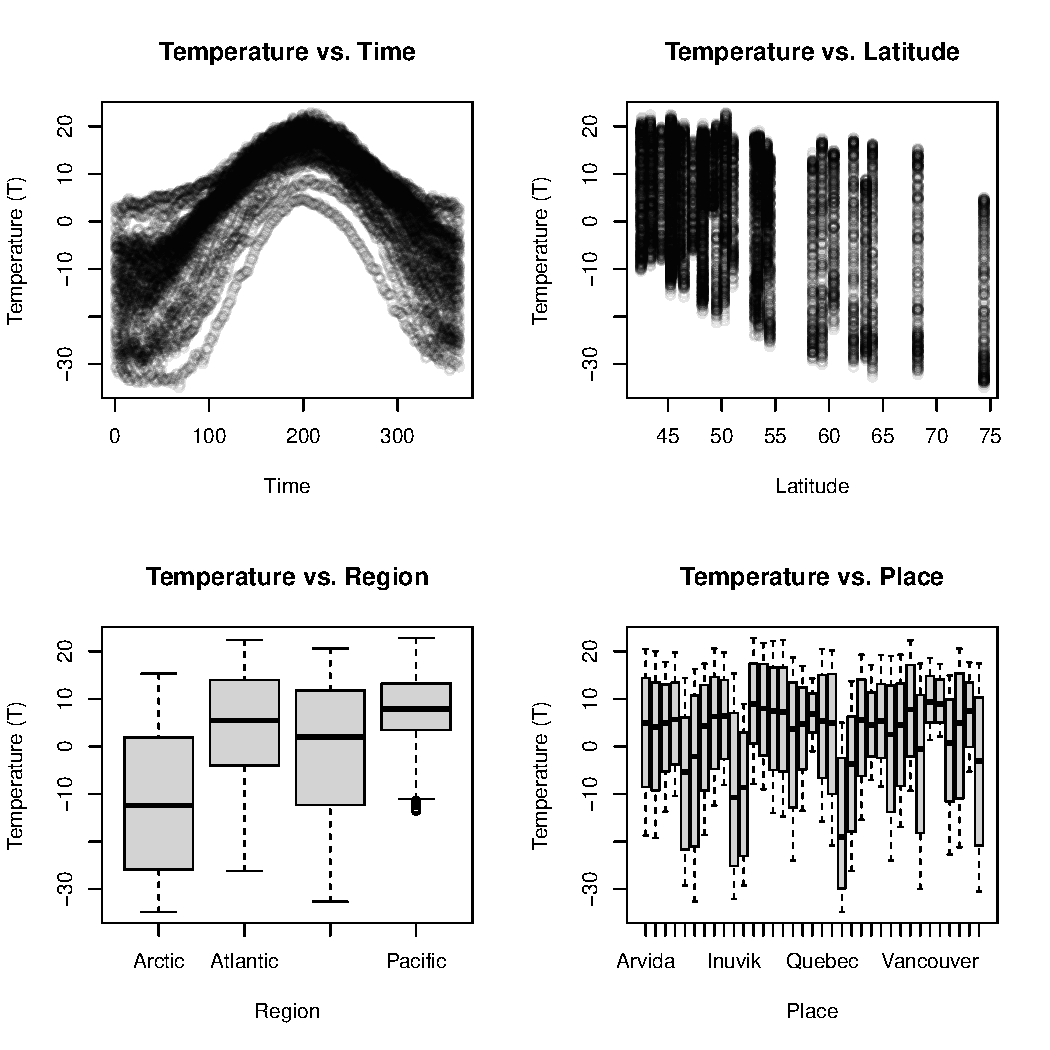
\includegraphics[width=0.99\linewidth,height=0.5\textheight]{figure/unnamed-chunk-3-1} 

}


\end{knitrout}

\section{Methods}\hfill\\

To simplify the analysis we implemented two types of approach: the first being a localized model and the second being a global model. By inspection, it can be seen that the data follows a clear bell-shaped distribution and so a direct observation was made to see a polynomial regression may have been suitable. Initial models indicated that a global polynomial fit was not suitable and un-interpretable. To account for this issue, we fit a polynomial model to each region hence mitigating the fitting problem:
$$\texttt{region\$T}\sim\texttt{Poly(region\$time, deg=6)}$$
Polynomials of degree 6 were used to fit the models since they are the lowest degree polynomials that provided sufficiently well enough fits for the data --- i.e., polynomials of lower degree did not fit the data well and polynomials of higher degree did not provide significant improvement in model fit for the corresponding computational costs.

With the additive models, we also fit in a similar manner of localizing a model to each region; but since the additive model can indeed incorporate regional indicators (specifically latitude) without losing significant goodness of fit, we also fit a global additive model with two covariates. This gives
$$\texttt{region\$T}\sim\texttt{Spline(region\$time)}$$
for the local spline regression model, and
$$\texttt{T}\sim\texttt{Spline(time, deg=3)}+\texttt{Spline(latitude, deg=3)}$$
for the global additive model. We use \texttt{mgcv}'s automatic selection feature to obtain our $\lambda$ values and knot counts for the additive models and it is important to note in the global additive model we use B-splines for smoothing \texttt{time} and cubic regression splines to smooth \texttt{latitude} for the purposes of a better fit.

In determining the goodness of the model fits, we will use the GCV estimates (expected generalization errors) and the adjusted R$^2$ values as these two statistics both are indicators for how well the model explains the data. The mean adjusted R$^2$ is used for the global additive model and the mean non-adjusted R$^2$ is used for all other models, since there is only one covariate in each of the localized models (adjusted and non-adjusted R$^2$ values are approximately equal) and we wish to be able to interpret the local R$^2$ values relative to the global model. As for the GCV estimates, \texttt{mgcv} provides GCV estimates for all the additive models, so we only have to compute the GCV estimate for the polynomial regression models; to be able to interpret these GCV estimates with respect to the global additive model results, we compute the GCV estimate by assuming the true temperature value to be the average temperature over each place in a region, that is
$$\texttt{true T at region r}=\frac{1}{\texttt{\# of places in r}}\sum_{\texttt{place in r}}(\texttt{T at place})$$
hence we will compute the fitted values in a similar manner to match the dimension of the true temperature value vector.

\section{Results}\hfill\\

Fitting our models to the data we get the following plots where the fitted line is in red and the confidence bands are in orange.
\begin{knitrout}
\definecolor{shadecolor}{rgb}{0.969, 0.969, 0.969}\color{fgcolor}

{\centering 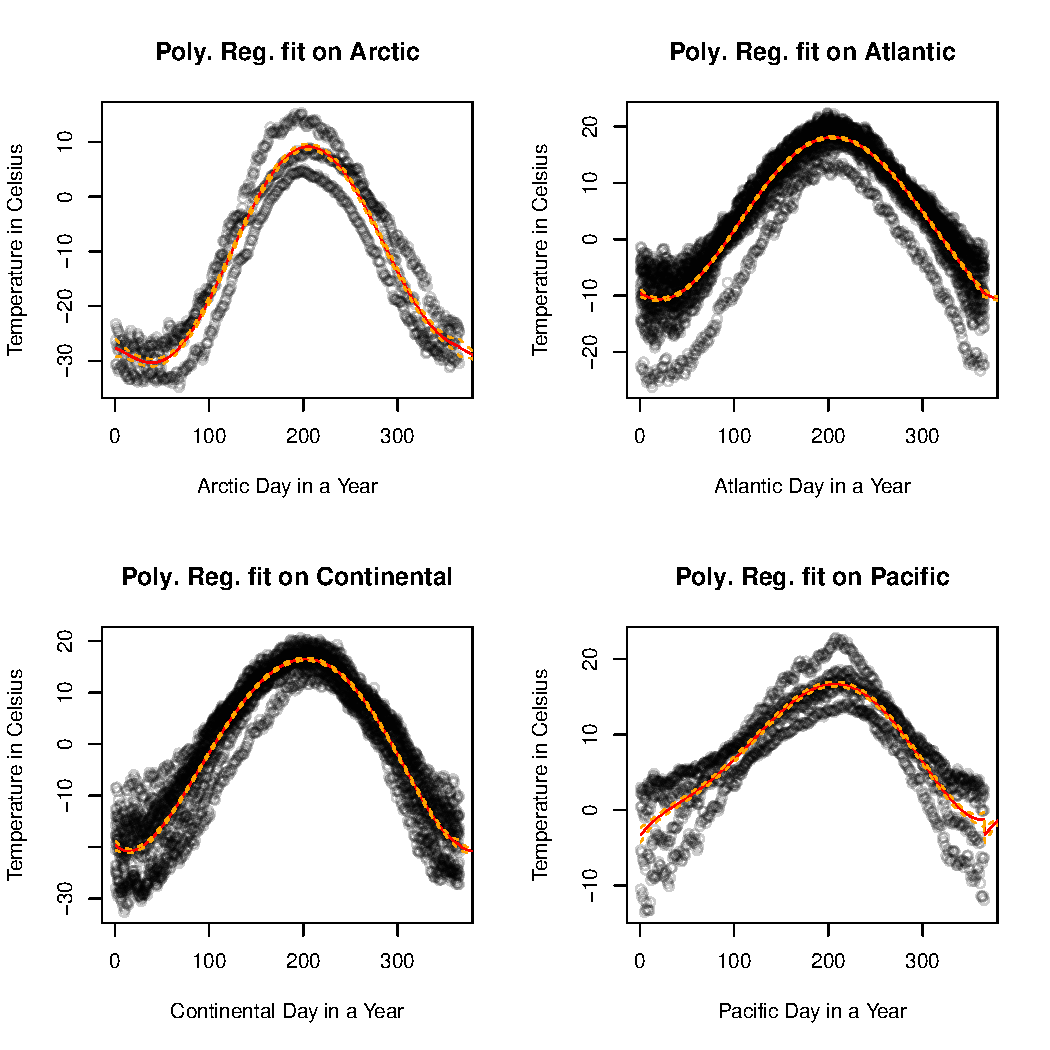
\includegraphics[width=1.01\linewidth,height=0.52\textheight]{figure/unnamed-chunk-4-1} 

}


\end{knitrout}

\begin{knitrout}
\definecolor{shadecolor}{rgb}{0.969, 0.969, 0.969}\color{fgcolor}

{\centering 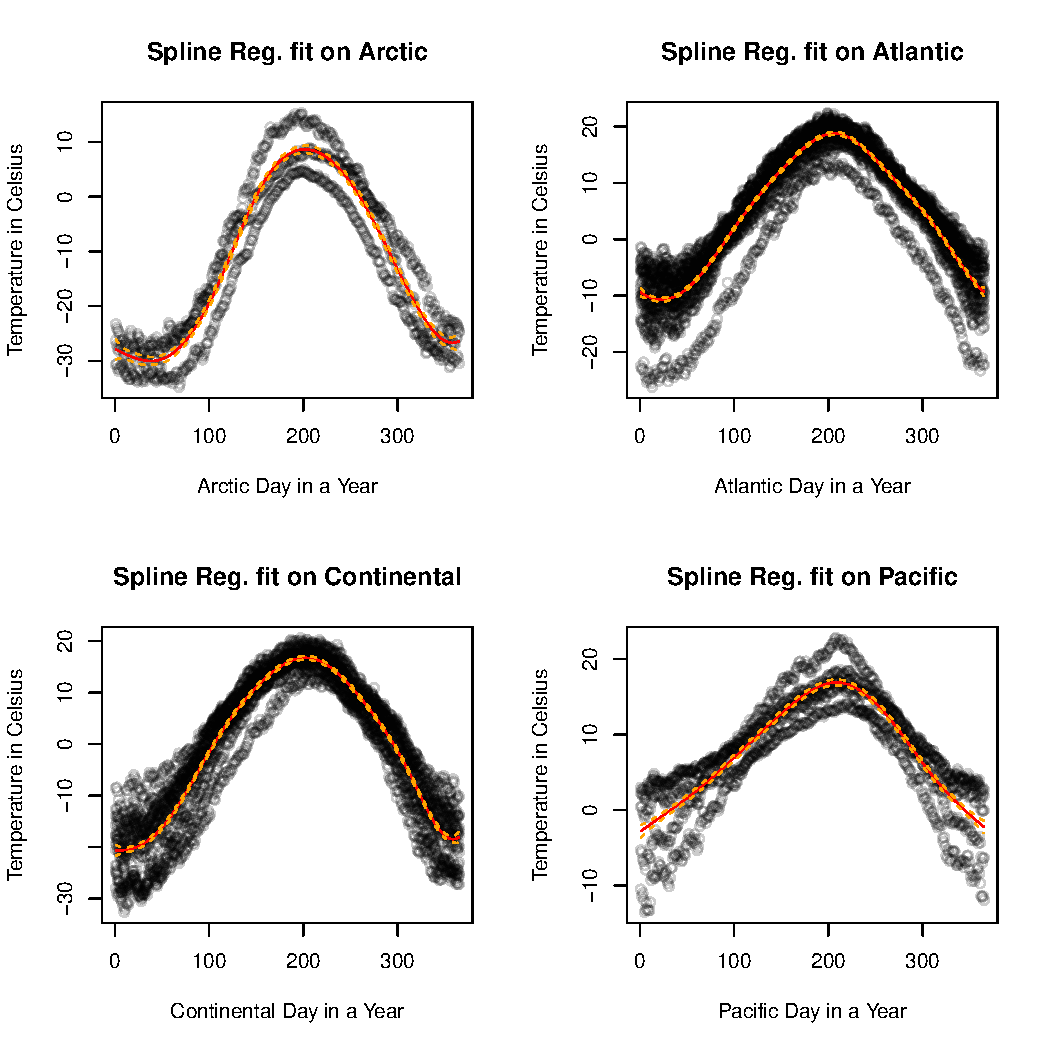
\includegraphics[width=1.01\linewidth,height=0.53\textheight]{figure/unnamed-chunk-5-1} 
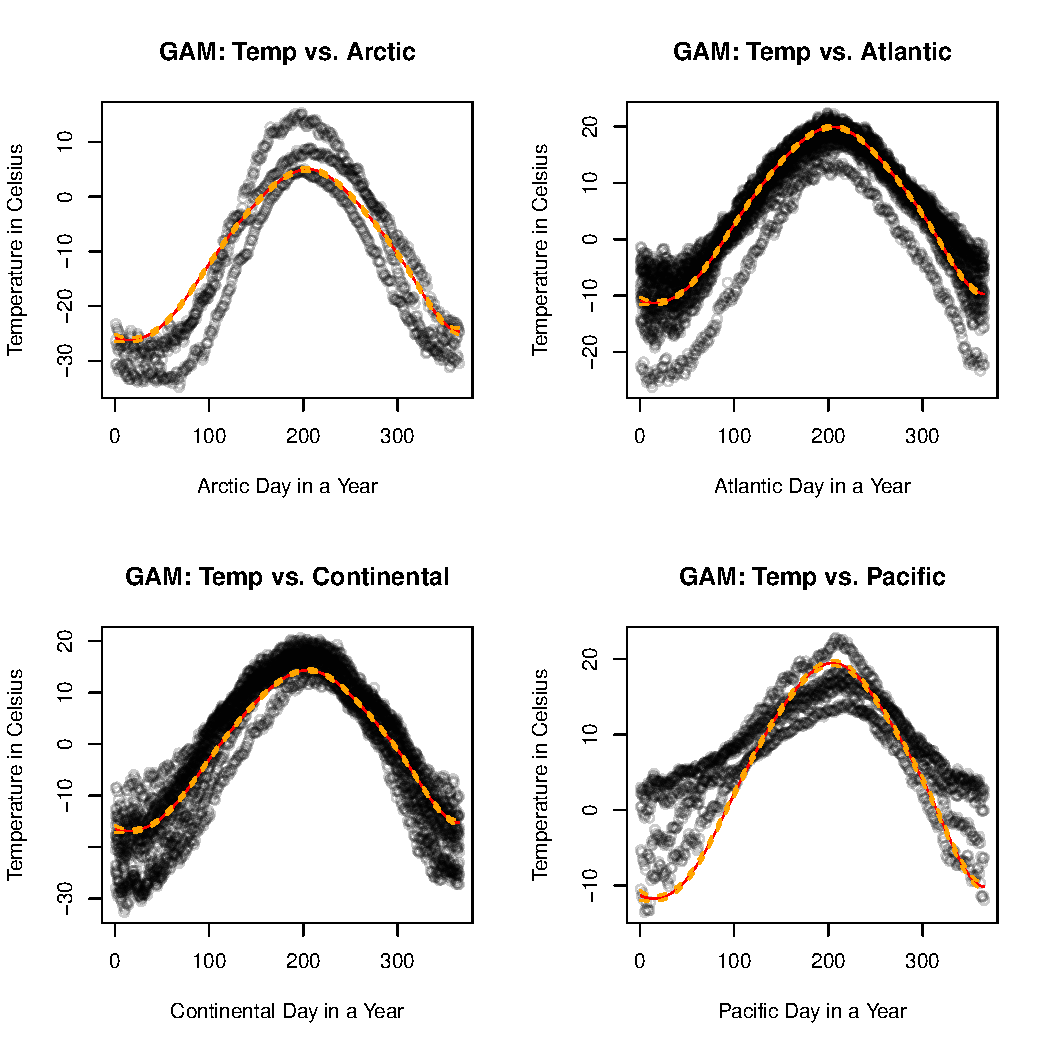
\includegraphics[width=1.01\linewidth,height=0.53\textheight]{figure/unnamed-chunk-5-2} 

}


\end{knitrout}

\noindent Notice the polynomial models when plotted out have these "jumps" nearing the end of the year --- the reason behind this requires a deeper understanding of the \texttt{R} functions used to fit and plot the models, however we suspect the reason behind this might be due to the repetition \texttt{time} (since it a sequence of numbers 1 to 365 repeated $n$ times for $n$ places in the region). Observe also that the plot of the global additive model for the Pacific region has a slightly higher amplitude than the two localized models. The cause of this is likely due to the fact that this model is fit globally, and since there is less data in the Pacific region than that of Continental and Atlantic, the influence of the trends in those two regions may have dominated that of the Pacific. Then to assess the goodness of fits, we compute the GCV estimates and R$^2$ values to get the results below.
\begin{knitrout}
\definecolor{shadecolor}{rgb}{0.969, 0.969, 0.969}\color{fgcolor}\begin{table}[!h]
\centering\begingroup\fontsize{11}{13}\selectfont

\begin{tabular}[t]{lrrr}
\toprule
  & Polynomial & Spline & GAM\\
\midrule
R squared & 0.87900 & 0.8794453 & 0.8916382\\
GCV estimate & 14.32027 & 14.2235375 & 17.8291651\\
\bottomrule
\end{tabular}
\endgroup{}
\end{table}

\end{knitrout}

Based on these values it can be concluded that while for the global additive model, the R$^2$ value is slightly better and the GCV estimate is slightly larger than that of the two localized models, in general there is minimal difference between the goodness of fit within each of the models.

\section{Conclusions}\hfill\\

While each method and corresponding model(s) fits to the data relatively well, we recall that the point of the study is an attempt to understand the spatial variance of annual Canadian temperature with respect to region; with this in mind, it is sensible to select the global additive model as our prime choice in understanding the data. This is because the global additive model not only provides easily interpretable results --- since we can plot out the partial effects and inspect the relationships between each covariate and \texttt{T} --- it also provides insight into national temperature patterns and not just regional patterns. In restricting our models to be local to a region, we gain minimal improvements in the goodness of fits at the cost of difficult and even un-interpretable results in which we cannot use to compare the relative spatial patterns of the annual temperature. It also makes it very difficult to understand the relationsip between each of the local models since each one is a separate model fit to one specific region, thus hindering the interpretability of the overall results. In addition, it is worth noting naive methods were implemented since the data used was relatively simple; if it were the case to see complicated and/or much larger amounts/types of data, other methods and models are recommended as they may be able to provide more accurate fits by taking into consideration more geological and meteorological phenomena.

\newpage


%%%%%%%%%%%%%%%%%%%%%%%%%%%%%%%%%%%%%%%%%%%%%%
%% Supplementary Material, including data   %%
%% sets and code, should be provided in     %%
%% {supplement} environment with title      %%
%% and short description. It cannot be      %%
%% available exclusively as external link.  %%
%% All Supplementary Material must be       %%
%% available to the reader on Project       %%
%% Euclid with the published article.       %%
%%%%%%%%%%%%%%%%%%%%%%%%%%%%%%%%%%%%%%%%%%%%%%
%\begin{supplement}
%\stitle{???}
%\sdescription{???.}
%\end{supplement}

%%%%%%%%%%%%%%%%%%%%%%%%%%%%%%%%%%%%%%%%%%%%%%%%%%%%%%%%%%%%%
%%                  The Bibliography                       %%
%%                                                         %%
%%  imsart-nameyear.bst  will be used to                   %%
%%  create a .BBL file for submission.                     %%
%%                                                         %%
%%  Note that the displayed Bibliography will not          %%
%%  necessarily be rendered by Latex exactly as specified  %%
%%  in the online Instructions for Authors.                %%
%%                                                         %%
%%  MR numbers will be added by VTeX.                      %%
%%                                                         %%
%%  Use \cite{...} to cite references in text.             %%
%%                                                         %%
%%%%%%%%%%%%%%%%%%%%%%%%%%%%%%%%%%%%%%%%%%%%%%%%%%%%%%%%%%%%%

%% if your bibliography is in bibtex format, uncomment commands:
\bibliographystyle{imsart-nameyear} % Style BST file
%\bibliography{bibliography}       % Bibliography file (usually '*.bib')

%% or include bibliography directly:
\begin{thebibliography}{1}
\bibitem[\protect\citeauthoryear{Environment and Climate Change Canada}{2023}]{b1}
\textsc{Environment of Canada} (2023). \textit{Canadian Environmental Sustainability Indicators: Temperature change in Canada}. Available at \href{https://www.canada.ca/en/environment-climate-change/services/environmental-indicators/temperature-change.html}{Canadian Environmental Sustainability Indicators: Temperature change in Canada}. Government of Canada.

\bibitem[\protect\citeauthoryear{Ramsay and Silverman}{2006}]{b2}
\textsc{Ramsay J.O. and B.W. Silverman} (2006). \textit{Functional Data Analysis}, 2nd ed. Springer.
\end{thebibliography}

\end{document}
